% Local alignment documentation fragment
%
% Figures and xrefs:
%   locality.tex:                2005/1126-document-localalignment
%   entryexit-example.[pdf,ai] : 2005/1024-labmeeting
% 

\documentclass[11pt]{article}

\usepackage{newcent}
\usepackage{mathptmx}
\usepackage{fullpage}
\usepackage{fancyvrb}
\usepackage{fancybox}
\usepackage[numbers,sort&compress]{natbib}
\usepackage[pdftex]{graphicx}
\usepackage[backref,colorlinks]{hyperref}

% customizations used in the User's Guide


% Description-like environment for documenting functions/APIs.
% puts the description label in a minipage with a large hanging
% indent.
% Good christ this took a long time to develop.
% hanging indent trick stolen from Peter Wilson's hanging.sty @CTAN
% minipage allows multi-line label, and puts item on next line.
% customized list inspired by Kopka/Daly _Guide to LaTeX_ p.213
% SRE, Wed Dec 27 11:37:18 2000
%
\newenvironment{sreapi}{%
     \begin{list}{}{%
       \renewcommand{\makelabel}[1]{%
         \begin{minipage}{\textwidth}%
           \hangindent10em\hangafter1\noindent%
           {\bfseries\texttt{##1}\vspace{0.8em}}%
         \end{minipage}%
     }}}%
     {\end{list}}


% Description-like environment for producing lists like:
%
%     label  stuff, stuff, stuff
%
%    label2  more stuff, more stuff,
%            more stuff.
% \begin{sreitems}{Longest label} \item[label] stuff, ... \end{sreitems}
% SRE, Wed Dec 27 11:59:43 2000
%
\newenvironment{sreitems}[1]{%
     \begin{list}{}{%
       \settowidth{\labelwidth}{#1}%
       \setlength{\leftmargin}{\labelwidth}%
       \addtolength{\leftmargin}{\labelsep}%
       }}
     {\end{list}}
       
\DefineVerbatimEnvironment{sreoutput}{Verbatim}{fontsize=\scriptsize,xleftmargin=2.0\parindent}%

\makeatletter
\newcommand{\listoffaqs}{\@starttoc{faq}}
\newenvironment{srefaq}[1]
{\addcontentsline{faq}{faq}{#1}\begin{sloppypar}\noindent\slshape\small\begin{quote}\textbf{$\triangleright$ #1}}
{\end{quote}\end{sloppypar}}
\newcommand{\l@faq}[2]{\@dottedtocline{0}{0pt}{0pt}{#1}{#2}}
\makeatother

% Consistent font styles
%   \software{} for the name of a software package
%   \database{} for the name of a database
%   \prog{}     for a program or file name
%   \emprog{}   for an emphasized program or file name
%   \user{}     for a typed user command
%   \response{} for an output line following a \user command
%
\newcommand{\software}[1]{\textsc{#1}}
\newcommand{\database}[1]{\textsc{#1}}
\newcommand{\prog}[1]{{\small\bfseries\texttt{#1}}}
\newcommand{\emprog}[1]{{\small\bfseries\texttt{#1}}}
\newcommand{\user}[1]{\indent\indent{\small\bfseries\texttt{> #1}}}
\newcommand{\response}[1]{\indent\indent{\small\bfseries\texttt{#1}}}

% The ``wideitem'' environment is mostly obsolete, but
% it gets used in converted manpages.
% 
\newenvironment{wideitem}{\begin{list} 
     {}
     { \setlength{\labelwidth}{2in}\setlength{\leftmargin}{1.5in}}}
     {\end{list}}

% The following are used as temp vars in how man pages are 
% converted into LaTeX w/ rman; see ``make manpages'' in Makefile.
%
\newlength{\sresavei}
\newlength{\sresaves}
\begin{document}

\section{A full probabilistic model of local alignment}

A \textbf{local alignment} is an alignment of a contiguous subsequence
$i..j$ of the target sequence to a contiguous subsequence $k..m$ of
the query. Traditionally, the flanking positions $1..i-1,j+1..L$ and
$1..k-1,m+1..M$ outside this local alignment not contribute to the
alignment score (or equivalently, can be considered to score zero).
In contrast, a \textbf{global alignment} algorithm finds an alignment
of the complete query and target, and any unaligned positions are
assessed insertion and deletion penalties. A \textbf{glocal} alignment
is global with respect to the query $1..M$, and local with respect to
a subsequence $i..j$ of the target. For example, this is useful when a
profile HMM defines a protein structural domain, which may occur in
the context of a longer protein sequence composed of several domains.

Local, global, and glocal alignment are traditionally described as
different algorithms that use the same scoring system.  For pairwise
sequence alignment, the canonical local alignment algorithm is the
\textbf{Smith/Waterman algorithm} \citep{Smith81}, and the canonical
global alignment algorithm is the \textbf{Needleman/Wunsch} algorithm
\citep{Needleman70}. Glocal alignment is a trivial hybrid of the two
algorithms \citep{Durbin98}. Essentially the same algorithms are
applied to position-specific profile scoring systems.

Our approach is essentially the opposite. We treat local versus global
alignment as a choice in model parameterization. A HMMER profile HMM
always explicitly models the complete target sequence, rather than
just identifying a high-scoring subsequence. An HMM state path can
include one or more local or global alignments to the model, plus
states that account for all nonhomologous residues of the target
sequence. A few extra state types and state transitions in the model
control local versus global alignment modes. The HMM algorithms used
to score and align target sequences (Forward and Viterbi) are
unaffected by whether the model is configured for local, global,
glocal, or other alignment styles.

Probabilistic models of local pairwise sequence alignment have been
described before, using pair-HMMs \citep{Durbin98,XXX}. The SAM
profile HMM software package explicitly models local, glocal, and
global alignment with states and state transitions, much as HMMER does
(though the SAM local alignment model is unnormalized). HMMER itself
has used an unpublished full probabilistic model of local alignment
since its inception in 1992. The specific ``Plan 7'' HMMER model
architecture we describe here has been in use since 1995. 

We therefore are not saying here that a full probabilistic model of
local alignment is a novel approach. Rather, it is an underappreciated
approach that has been reinvented by different people in different
guises. We will take some time to introduce the approach, and to
illuminate its reinventions. 

We have also found that the exact parameterization of local alignment
modes is surprisingly important. 


\section{Terminology}

Readers familiar with profile HMM applications and probabilistic
inference may skim or skip this section, which introduces a relatively
familiar notation \citep{Durbin98}.

The problem is \textbf{similarity search}. We are interested in
identifying whether a given target sequence $\mathbf{x}$ is homologous
to a query \textbf{profile}, or not. The profile is typically a
position-specific scoring model of a multiple sequence alignment of a
known sequence family. In the special case where the profile is
parameterized from a single sequence, the profile search is identical
with standard pairwise similarity search methods (such as BLAST).  We
will apply the search to every sequence in a target sequence database,
one at a time.




Homology is qualitative, not quantitative. A sequence is either
related to our query sequence(s) by common descent, or it is not.
However, our confidence in calling the target sequence homologous or
not may be expressed quantitatively. Using posterior probabilities to
express a degree of belief is a hallmark of Bayesian probabilistic
inference.

Additionally, our approach is not limited to strict evolutionary
homology....




\subsubsection{Probabilistic inference and probabilistic models}

We take a \textbf{probabilistic inference} approach. To determine how
probable it is that the sequence $x$ is homologous to our query,

\begin{equation}
   P(H \mid \mathbf{x} = \frac{P(\mathbf{x} \mid H) P(H)}
                           {\sum_{H'} P(\mathbf{x} \mid H') P(H')}
\end{equation}

To do the summation in the denominator, we must specify not only the
hypothesis $H$ that the sequence is homologous to the query, but all
possible alternative hypotheses $H'$ that might account for the
sequence. A standard simplification is to assume a single \textbf{null
hypothesis}, $R$, which generates random (independent, identically
distributed) nonhomologous sequences. The posterior then becomes:

\begin{equation}
   P(H \mid \mathbf{x}) = \frac{P(\mathbf{x} \mid H) P(H)}
                           {P(\mathbf{x} \mid H) P(H) P(\mathbf{x} \mid R) P(R)}
\end{equation}

Equivalently, we can define a log-odds score $s$:

\begin{equation}
  s = \log \frac{P(\mathbf{x} \mid H)} {P(\mathbf{x} \mid R)}
\end{equation}
 
which is related to the posterior probability by a sigmoid function:

\begin{equation}
  P((H \mid \mathbf{x}) = \frac{e^{s+c}} {1 + e^{s+c}}
\end{equation}

where $c$ is a constant that is the log of the prior odds ratio, $\log
\frac{P(H)}{P(R)}$.

Reporting log-odds scores $s$ instead of posterior probabilities is
convenient, because we are used to seeing scores from other standard
sequence alignment tools (such as BLAST). Substitution score matrices
are explicitly calculated as log-odds scores.  Additionally, Altschul
has shown that at least for ungapped alignment, even ad hoc score
matrices imply log-odds scores and an implicit target and background
probability model \citep{Altschul91}.

However, in standard approaches, only residue scores are derived
probabilistically, and remaining parameters (such as gap penalties and
the cost for starting/ending a local alignment) are arbitrary, so a
traditional alignment score cannot be readily interpreted as a
posterior probability. A score is therefore an arbitrary statistic.
To know whether a score should be interpreted as evidence that the
target sequence is homologous to the query or not, the statistical
significance of the score must be evaluated by calculating the
expected number of hits that would be expected to have this score or
greater if the entire target sequence database were nonhomologous
random sequences. A principal breakthrough that led to the popularity
of the BLAST suite of programs was \textbf{Karlin-Altschul
statistics}, the proof by Dembo, Karlin, and Altschul that ungapped
sequence alignment scores follow an extreme value (Gumbel)
distribution, and subsequent empirical demonstrations that reasonable
gapped alignment scores are also Gumbel distributed.

In a probabilistic inference approach, ideally there would be no need
for any evaluation of the ``statistical significance'' of the score
$s$.  The log odds score is not an arbitrary statistic. It is directly
interpretable as the posterior probability we want to measure -- quite
literally the probability that our target sequence is homologous to
our query or not. For this to be true, though, we must be rigorous in
demanding that both $H$ and $R$ are full probabilistic models, with no
arbitrary (non-probabilistic) scores.

That is, by definition, $P(\mathbf{x} \mid H)$ and $P(\mathbf{x} \mid
R)$ must sum to one over all possible sequences $\mathbf{x}$.  (When
we emphasize \emph{full} probabilistic models, we mean models that are
correct in this respect, as opposed to approaches that use some
probabilistic justification for their scores.)  Because there are an
infinite number of sequences $\mathbf{x}$ of all possible lengths, but
we would rather have a finite number of parameters in our models, we
use \textbf{generative probabilistic models} to specify these
distributions. Specifically, for the case of linear primary sequence
profiles, where we are willing to assume that individual residues are
statistically independent of each other, we use a well-known class of
models called \textbf{hidden Markov models (HMMs)} \citep{Durbin98}.


\subsection{Profile hidden Markov models: definitions}

Without loss of generality, we will only discuss protein sequence
analysis, and an alphabet of $K=20$ amino acid residues. The same
approaches apply to DNA or RNA sequence analysis.

The \textbf{query} is a profile hidden Markov model (profile HMM)
called $H$. This model is built from a multiple sequence alignment of
homologous protein sequences, with position-specific residue
probabilities and indel probabilities for $N$ consensus aligned
columns. (The query $H$ may also be built from a single sequence, in
which case a profile HMM method is the same as pairwise sequence
alignment \citep{HolmesBruno01}.)

The \textbf{target} is a single sequence $\mathbf{x}$ of length $L$,
with residues $x_1..x_L$. 

A \textbf{state path} (or just \textbf{path}) $\pi$ consists of a
sequence of $P$ states $\pi_1..\pi_p..\pi_P$ that describe a path
through the profile HMM that could generate the target sequence
$\mathbf{x}$. Because the profile HMM will contain some mute states
that do not emit any residues, $P$ is greater than $L$. (Unlike
canonical HMMs, whose states always emit one residue, and for which
$P=L$.) A path $\pi$ is equivalent to the more traditional notion of
an \textbf{alignment} of the profile to the target sequence.  





The \textbf{Viterbi algorithm} is a dynamic programming algorithm that
finds the optimal (highest probability) path, $\argmax_\pi
P(\mathbf{x}, \pi \mid H)$.

The \textbf{Forward algorithm} is a dynamic programming algorithm that
finds the marginal probability of the sequence given the model
$P(\mathbf{x} \mid H)$, which is a sum over all possible paths that
could generate that sequence, $P(\mathbf{x} \mid H) = \sum_\pi
P(\mathbf{x}, \pi \mid H)$. 

Viterbi and Forward are standard HMM algorithms. For the general case
of HMMs of $N$ states fully connected by an $N \times N$ transition
matrix, these algorithms require $O(LN)$ memory and $O(LN^2)$ time.
For the specific case of linear profile HMMs, which have a constant
number of transitions per state (no more than 4, in the case of
HMMER's architecture), they are $O(LN)$ in both time and memory.
















There are a number of reasons why local alignment is important, and
global alignment is not generally useful. ...

\subsection{Probabilistic models}

A \textbf{probabilistic model} of the target sequence $\mathbf{x}$
assigns


... Because there are an infinite number of possible sequences
$\mathbf{x}$ when indels are allowed, it is important to  ...



\subsection{HMMER's profile HMM architecture}




\subsubsection{The HMM: the core model}

%% Insert figure of the core profile.

The \textbf{core model} is a generative probabilistic model of global
sequence alignment. It consists of match (M), delete (D), and insert
(I) states, plus a special begin state (B) and end state (E).

Each consensus column $1..k..M$ of a multiple alignment is assigned to
one \textbf{node} consisting of a M, D, and I state triplet. The $M_k$
state generates a residue according to emission probabilities
estimated from consensus column $k$. The $I_k$ state emits one or more
residues inserted between consensus columns $k$ and $k+1$. The $D_k$
state is mute (that is, it does not emit a residue), allowing a
residue in column $k$ to be skipped (a deletion relative to
consensus).

This design essentially follows the profile HMM architecture
introduced by Krogh \emph{et al.}  \citep{Krogh94}. The main
difference is that $D_k \rightarrow I_k$ and $I_k \rightarrow D_{k+1}$
transitions are omitted by HMMER. The Krogh/Haussler model has nine
transitions per node, whereas HMMER has seven. Internally, we call the
HMMER architecture ``Plan 7''.

All paths through the profile core (samples from $P(x, \pi \mid H)$)
must visit either a match or delete state in every position $k$.
Every residue $x_i$ in the emitted sequence is assigned to either a
match or an insert state.

The core model is implemented in the \ccode{P7_HMM} structure in
\ccode{plan7.h}:

\begin{cchunk}
  int     M;                    /* length of the model (# nodes)          */
  int     K;			/* alphabet size (copy of Alphabet_size)  */
  float **t;                    /* transition prob's. t[(0),1..M-1][0..6] */
  float **mat;                  /* match emissions.  mat[1..M][0..K-1]    */ 
  float **ins;                  /* insert emissions. ins[1..M-1][0..K-1]  */
\end{cchunk}


\subsection{A profile: the search/scoring model}

The \textbf{search model} (\textbf{profile}) differs from the core
model in two respects. First, it contains scores, not probabilities.
Second, it has extra states and state transitions that enable it to
model glocal and local alignments.

The search model always corresponds to a generative probabilistic
model. However, it may not be exactly the model shown in Figure~{xxx},
because of a technicality in how I handle local alignment with respect
to the model. Generating sequences from a search model (sampling
sequences from the distribution $P(x \mid M)$) requires special
handling of begin/exit transitions, as described below (XXX).


\subsubsection{Locality with respect to the model}

In the search model, the $B \rightarrow M_k$ \textbf{entry}
probabilities and the $M_k \rightarrow E$ \textbf{exit} probabilities
specify a probabilistic model of local alignment with respect to the
model. That is, a path can generate a subsequence of the model by
using these transitions. 

In what follows, let $b_k$ represent the $B \rightarrow M_k$ entry
probabilities, and let $e_k$ represent the $M_k \rightarrow E$ exit
probabilities. The $b_k$'s are a probability distribution, summing to
one over all $k : 1 \leq k \leq N$. The $e_k$ probabilities are not a
probability distribution; instead, each is a new transition added to
the state transition distribution for state $M_k$. When the local
algorithm mode imposes a nonzero $e_k$ probability, the other $M_k$
transitions are renormalized to sum to $1-e_k$.

How should these entry and exit probabilities be set, when we allow
local alignment with respect to the model? I assume an uninformative
\textbf{uniform distribution} over all possible fragments $k..m$. I
will show that this corresponds to the implicit assumption of the
Smith/Waterman algorithm, up to a constant. Because there are
$N(N+1)/2$ possible fragments $k..m$ for a model of $N$ consensus
match states, the probability of each fragment will be set to
$2/N(N+1)$. HMMER uses some trickery to achieve this desideratum
within the constraints of the search model's architecture.

It is not sufficient to set a uniform entry probability distribution
($b_k = \frac{1}{N}$) and a constant exit probability $e_k = c, k <
N$. The exit probability from $M_N$ is 1.0 by definition, and
renormalization of the $M_k$ transition distributions means a
probability of $(1-c)$ for \emph{not} exiting from each successive
internal match state in a path. Therefore, in the extremes, the
fragment $N..N$ would occur with probability $\frac{1}{N}$, and
fragment $1..N-1$ would occur with probability $\frac{c
(1-c)^{N-2}}{N}$ (roughly speaking, ignoring other transition
probabilities involving deletes and inserts). Thus local alignments
that end at the last match state would be favored, especially shorter
alignments that enter close to that state.\footnote{HMMER2 configured
local alignment entry/exit probabilities in essentially this way,
albeit not quite this badly biased (the exit probabilities were not
constant, partially compensating for the fragment bias). The
non-uniform, strongly right-end-biased distribution that resulted was
pointed out as a potential problem by both Bob Edgar and Bill Bruno.}

Suppose we had a model that consisted solely of $N$ match states, with
no delete and insert states. Bill Bruno (personal communication)
observed that there is a unique solution for the entry and exit
probabilities that achieves a uniform fragment distribution:

\begin{eqnarray*}
   b_k & = & \frac{2(N-k+1)}{N(N+1)}\\
   e_k & = & \frac{1}{2(N-k+1)}
\label{eqn:uniform-entryexit}
\end{eqnarray*}

These are derived by recursively solving for our desideratum:

\begin{eqnarray*}
   b_k
   \left[\prod_{s=k}^{m-1} (1-e_k) \right]
   e_m
   = \frac{2}{M(M+1)}
\end{eqnarray*}

for all possible fragments $k..m$, starting from an initial constraint
that $e_N = 1.0$.

An example is shown in Figure~\ref{fig:entryexit-example}.

\begin{figure}
\begin{center}
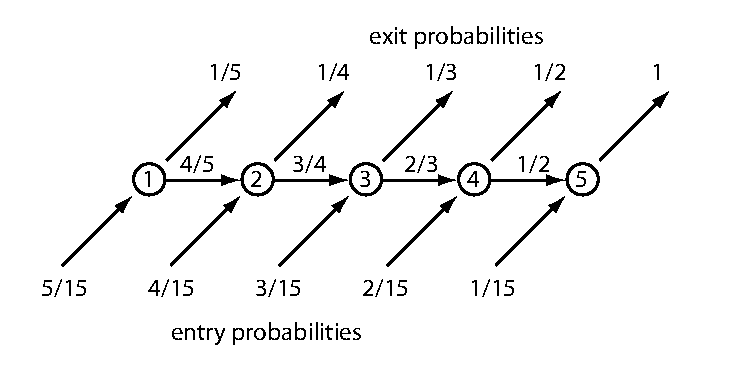
\includegraphics[width=4.5in]{entryexit-example}
\end{center}
\caption{\textbf{Entry and exit probabilities that achieve a uniform
fragment distribution for a model consisting solely of match states.}
Values are shown for entry, exit, and match $\rightarrow$ match state
transition probabilities (arrows) are shown for an example of a model
of 5 consensus match states, as specified by
Equation~\ref{eqn:uniform-entryexit}.}
\label{fig:entryexit-example}
\end{figure}

This elegant solution is complicated by the presence of delete states
in the model. I do not allow a local alignment to end from a delete
state, so $D_k \rightarrow D_{k+1}$ transitions are not subject to the
$(1 - e_k)$ renormalization imposed on $M_k$ transitions. This will
create a bias towards local alignment paths that contain deletions.

HMMER therefore subtracts the $\log(1-e_k)$ renormalization term from
\emph{both} the delete transition scores and the match transition
scores. This guarantees that any transition from node $k \rightarrow
k+1$ is assessed one $\log(1-e_k)$ term. Any local alignment path that
starts in node $k$ and ends from node $m$ will be assessed the correct
$\log(\frac{2}{N(N+1)})$ total log probability for locality, no matter
how many delete states are used. In the source (\ccode{modelconfig.c})
this step is called \textbf{D-path leveling}.

Thus when a HMMER search model is in its default local alignment mode
(not global or glocal modes, or custom modes that use the full
probabilistic search model without the D-path leveling trick), the
search profile does not correspond exactly to the generative
probabilistic search model shown in Figure~xxx. Nonetheless, the
profile scores do correspond to a generative probabilistic model, one
in which the start and end points $M_k,M_m$ are drawn uniformly from
all ${N(N+1)}{2}$ possible fragments $k..m$, and then a path that
starts at $M_k$ and ends at $M_m$ is sampled. The long-range
dependence of $k,m$ is hard to model as an HMM;
Figure~\ref{fig:implicit-local} shows how it would be done, by
replicating all the model fragments explicitly. The score of every
path in this model is provably identical to the score of the
corresponding path in HMMER's search profile, therefore this is the
probabilistic model implied by the scores of a HMMER search profile in
local alignment mode.

\begin{figure}
\begin{center}
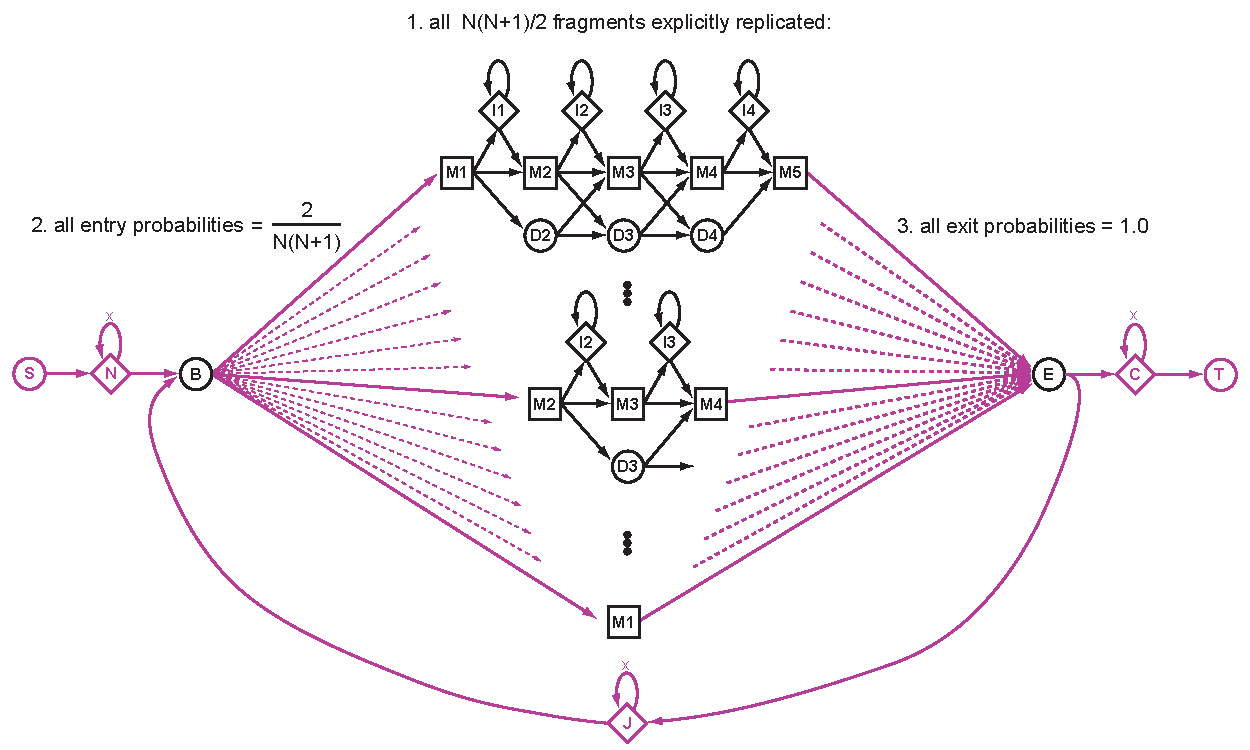
\includegraphics[width=5in]{implicit-local}
\end{center}
\caption{The generative probabilistic model of local alignment
implicit in a HMMER search profile's transition scores, when D-path
leveling is used to assure uniform fragment length distribution.}
\label{fig:implicit-local}
\end{figure}

To correctly sample sequences from a local profile, the following
sampling procedure is used:

\begin{itemize}
\item Sample start and end $k,m$ from a uniform distribution over all
      $N(N+1)/2$ choices for $k \leq m$.  One way to do this is by
      rejection sampling: sample $k$ and $m$ uniformly on the interval
      $1..N$, reject any pair $k>m$, repeat until acceptance.\footnote{HMMER
      uses a more efficient algorithm based on a transformation of the
      triangular matrix $k \leq m$ to a vector.}

\item Sample a path that starts from $M_k$ and ends in $M_m$ by
      rejection sampling, as follows: start in $M_k$, use the usual
      HMM generation algorithm (with the core HMM's transition and
      emission probabilities) to choose transitions and emissions
      until the path reaches node $m$; if the chain is in delete state
      $D_m$, reject the path; repeat until a path ends in $M_m$.
\end{itemize}


\subsection{Locality with respect to the target sequence}


\subsection{Wing retraction}

In order to avoid a mute cycle (a subpath consisting solely of
nonemitting $B$, $D$, and $E$ states and no $J \rightarrow J$
transition), HMMER eliminates the $D_1$ and $D_N$ states as the first
step in the process of configuring the search model from the core
profile. This is called ``wing retraction''. 
\footnote{The term is an analogy to swing-wing aircraft in
takeoff/landing mode versus high speed flight. Swing-wing aircraft,
typified by the US F-14 Tomcat and F-111 Aardvark, were in vogue a
decade or so ago, but the complexity and weight of such designs are
currently thought to outweigh any advantages
[\url{http://en.wikipedia.org/wiki/Swing-wing}]. This is also the case
for wing retraction in HMMER, but wing retraction is deeply embedded
in the current code design.}

Wing retraction does not significantly alter the probabilistic
model. The mute cycle itself is deemed impossible, so its probability
is removed and the model is renormalized. This has a negligible effect
for all but the shortest models. All the remaining probability that
flows through $D_1$ and $D_N$ in the core model is accounted for
exactly by an alternative representation in the search model: all
paths that would have utilized the $D_1$ state are accounted for by
direct $B \rightarrow M_k$ internal entries, and all paths that would
have utilized the $D_N$ transition are instead accounted for by $M_k$
internal exits.

Specifically, we calculate a probability $bm_k$ of all delete-only
path segments $B \rightarrow D_1 ... D_k-1 \rightarrow M_k$ that use
$D_1$ and end in a match state $M_k$ in the core model, for all $k>1$:

\begin{equation}
   bm_k = t(B \rightarrow D_1) \cdot
            \left[ \prod_{j=2}^{k-1} t(D_{j-1} \rightarrow D_j) \right] \cdot
            t(D_{k-1} \rightarrow M_k)
\end{equation}

and a probability $m_ke$ of all delete-only path segments $M_k
\rightarrow D_{k+1}...D_N \rightarrow E$ that start with $M_k$ and end
in $E$ in the core model, for all $k<N$:

\begin{equation}
   mk_e = t(M_k \rightarrow D_{k+1}) \cdot
            \left[ \prod_{j=k+2}^{N} t(D_{j-1} \rightarrow D_j) \right] 
\end{equation}

We also calculate the probability of the mute (all-delete) path
through the entire model from $B$ to $E$:

\begin{equation}
  p_{\mbox{mute}} =  t(B \rightarrow D_1) \cdot
       \left[ \prod_{j=2}^{N} t(D_{j-1} \rightarrow D_j) \right] 
\end{equation}

($t(D_N \rightarrow E)$ is 1.0 by definition, so it does not appear in
the last two equations.)

What we do with these subpath probabilities depends on whether the
model is being configured for glocal alignment or local alignment. 

In a glocal mode, where no algorithm-dependent internal entry is
permitted, the search model's $t(B \rightarrow M_k)$ internal entry
probability is set to $bm_k$ for $k>1$, and the $t(M_k \rightarrow E)$
internal exit probability is set to $m_ke$ for $k<N$. The internal
entry probabilities (which sum to $1-p_{mute}$) are then renormalized
by dividing through by $1-p_{mute}$.  Use of an ``internal'' entry
transition by a glocal model is then interpreted as a use of the
equivalent all-delete path from $B \rightarrow D_1 ... D_{k-1}
\rightarrow M_k$, and an ``internal'' exit is interpreted as an
all-delete path $M_k \rightarrow D_{k+1}...D_N \rightarrow E$.

In a local mode, the subpath probabilities are discarded, and
overridden by the algorithm-dependent internal entry and exit
probabilities imposed by local mode (as described below). In local
mode, a path through the core model may not begin or end with delete
states at all. The uniform fragment length distribution imposed by a
local algorithm mode supersedes whatever the profile core thinks it
has learned about fragment lengths (terminal $D \rightarrow D$
prefixes and suffixes) from the multiple sequence alignment the core
model was built from.

This removal of a formally problematic mute cycle is more stylistic
than functional. Equivalently, we could simply ignore the probability
lossage that results because the Viterbi and Forward algorithms cannot
capture mute cycles. 

% Discuss how to train on fragments.
















%% equivalence between path and alignment. Define \pi.







We could achieve local alignment simply by applying the Smith/Waterman
algorithm, with the core profile providing our scoring system, but the
result would no longer be a correct probabilistic model. That is, if
we allow an alignment to start or end at any internal position $k$
with zero cost, as in Smith/Waterman, this is equivalent ...



\subsection{Discussion}

\subsection{Traditional scoring}

Traditionally, pairwise sequence alignments are scored using a $20
\times 20$ \textbf{substitution matrix} to score aligned residue
pairs, and \textbf{gap-open} and \textbf{gap-extend} penalties for
scoring insertions and deletions. For example, the popular WU-BLAST
program scores amino acid sequence alignments with the BLOSUM62
substitution matrix and gap penalties of -9/-2. 

Substitution matrices are understood...

\subsection{Other probabilistic alignment approaches}

Yu and Hwa wrote that ``probabilistic alignments lead to anomalous
[non-Gumbel] statistics'' \citep{YuHwa01}. In saying this, they
confused the model with the choice of alignment algorithm. We will
show here that probabilistic local optimal alignment (the Viterbi
algorithm) yields Gumbel statistics.  What Yu and Hwa call
``probabilistic sequence alignment'' is the Forward algorithm (which
is not an alignment algorithm). We confirm here that Forward scores
are not Gumbel-distributed.

% check Bucher/Hofmann reference

Some ``probabilistic'' alignment methods start with arbitrary scores
and treat them as unnormalized log probabilities or pseudoenergies
that can be converted to probabilities via a Boltzmann-Gibbs partition
function \citep{ZhangMarr95,BucherHofmann96,YuHwa01}. A disadvantage
of these approaches is that the resulting probability distribution
$P(x \mid M)$ is only indirectly related to the scoring system, via
relatively complex calculations.

%% Also here: Holmes 98; Miyazawa 84; perhaps TKF and Bishop/Thompson

\subsection{Comparison to SAM}

HMMER's N and C states are essentially equivalent to ``free insertion
modules'' (FIMs) that SAM uses to achieve locality with respect to the
target sequence. To achieve locality with respect to the model, SAM
allows internal entry/exit transitions with probability 1.0. 

\bibliographystyle{abbrv}
\bibliography{master,lab,books}
\end{document}